\documentclass[12pt,a4paper]{report}
\usepackage{graphicx}
\usepackage{amssymb,amsmath,amsthm}
\usepackage{pgfplots}
\usepackage{comment}

\newtheorem*{theorem1}{Performance of GPU passthrough}
\newtheorem*{theorem2}{Driver compatability}

\pgfkeys{/pgfplots/axis labels at tip/.style={
    xlabel style={at={(current axis.right of origin)}, xshift=1.5ex, anchor=center},
    ylabel style={at={(current axis.above origin)}, yshift=1.5ex, anchor=center}}
}

\begin{document}
\begin{titlepage}
	\centering
	{\scshape\LARGE HTL Spengergasse \par}
	\vspace{1cm}
	{\huge\bfseries GPU Passthrough in ESXi \par}
	\vspace{1.5cm}
	{\scshape\Large Setup and comparison of performance \par}
	\vspace{2cm}
	{\Large\itshape Florian \textsc{Schaar} and Ariel \textsc{Simulevski}\par}
	\vfill
	supervised by\par
	Hans-Peter \textsc{Berger}

	\vfill

% Bottom of the page
	{\large \today\par}
\end{titlepage}

\newpage

\tableofcontents

\newpage

\chapter{Introduction and theorems}

\section{Introduction}

As virtual machines and decentralized architecture become increasingly important and the need for dispersed, high performance computing rises, native, low overhead GPU performance is becoming a necessity for datacenter applications, especially in deep-learning, remote rendering and blockchain usecases. With GPU passthrough, exactly that can be achieved while being efficient and manageable.

\section{Theorems}

\begin{theorem1}
When a PCIe graphics device is forwarded to a virtual machine, the performance difference should be minimal due to the fact that the CPU still uses the same interfaces and buses when running in a virtual machine with VT-d enabled.
\end{theorem1}

\begin{theorem2}
GPU passthrough on ESXi should be compatible with all devices which support OpenGL, since this is a open source library and implements a graphics-interface standard.
\end{theorem2}

\chapter{Setup}

\section{Requirements}

\begin{enumerate}
\item A system with ECC memory
\item An ESXi installation
\item A PCIe based graphics device (tested with NVIDIA and AMD devices)
\end{enumerate}

\section{Setup}

After creating a new virtual appliance on the system, one needs to enable the passthrough option for the according PCIe device. It is advised to also enable said option for the audio controller/device of the PCIe graphics device. After rebooting the host-system, one can add the previously mentioned device to the virtual machine in the appliance-settings.
\newline
Important:
\begin{enumerate}
\item "Reserve all guest memory" has to be enabled
\item Add the device as a PCI/PCIe device
\item Under all circumstances, avoid adding the audio device to the appliance as this might cause unknown behavior
\end{enumerate}
Now, one can install their operating system of choice. After this installation process is done, install the appropriate drivers for the graphics device.

\chapter{Benchmark and conclusion}

\section{Cinebench GPU Benchmark}

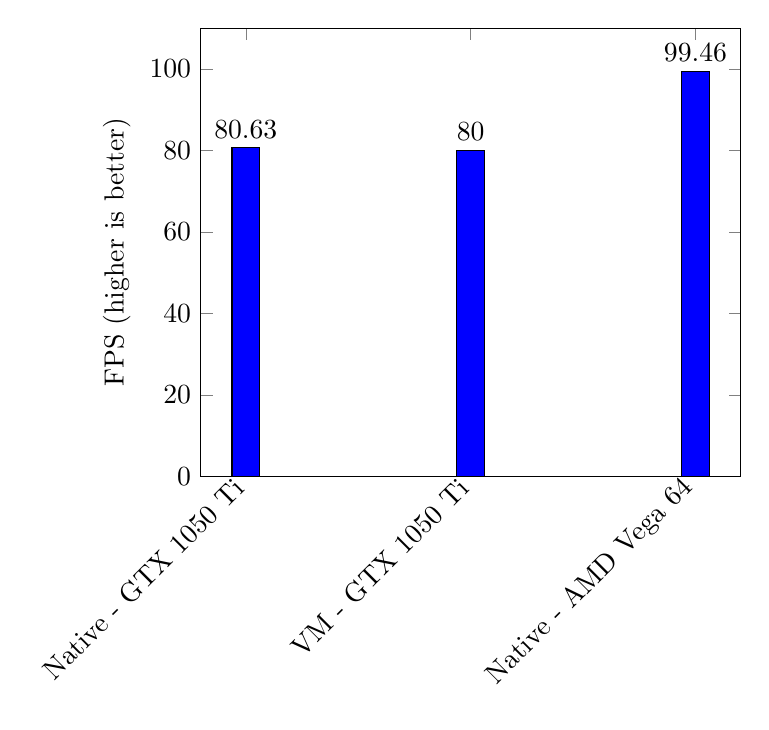
\begin{tikzpicture}
  \begin{axis}[
	ylabel=FPS (higher is better),
	ymax=110,
	ymin=0,
	symbolic x coords={Native - GTX 1050 Ti,VM - GTX 1050 Ti,Native - AMD Vega 64},
    xtick=data,
    x tick label style={rotate=45, anchor=east},
    nodes near coords
  ]
    \addplot [ybar,fill=blue]
    	coordinates {
    		(Native - GTX 1050 Ti,80.63)
			(VM - GTX 1050 Ti,80.0)
			(Native - AMD Vega 64, 99.46)
		};
  \end{axis}
\end{tikzpicture}

\begin{comment}
 TODO: Add real benchmark for 'VM - GTX 1050 Ti'
\end{comment}

\section{Conclusion}

GPU passthrough is a very mighty tool and a great feature of ESXi. However, it has to be taken with a grain of salt, as it introduces many new problems, unknown behavior and potentially, bugs. Furthermore, the feature is not compatible with all cards. Usage on a bigger scale has to be evaluated further.

\begin{comment}
 TODO: Add conclusion for Theorems
\end{comment}

\end{document}
